% Slide 17 — Nenhuma política domina simultaneamente
\begin{frame}{Nenhuma política domina simultaneamente}
  \begin{columns}[T,onlytextwidth]
    \column{0.5\textwidth}
      \centering
      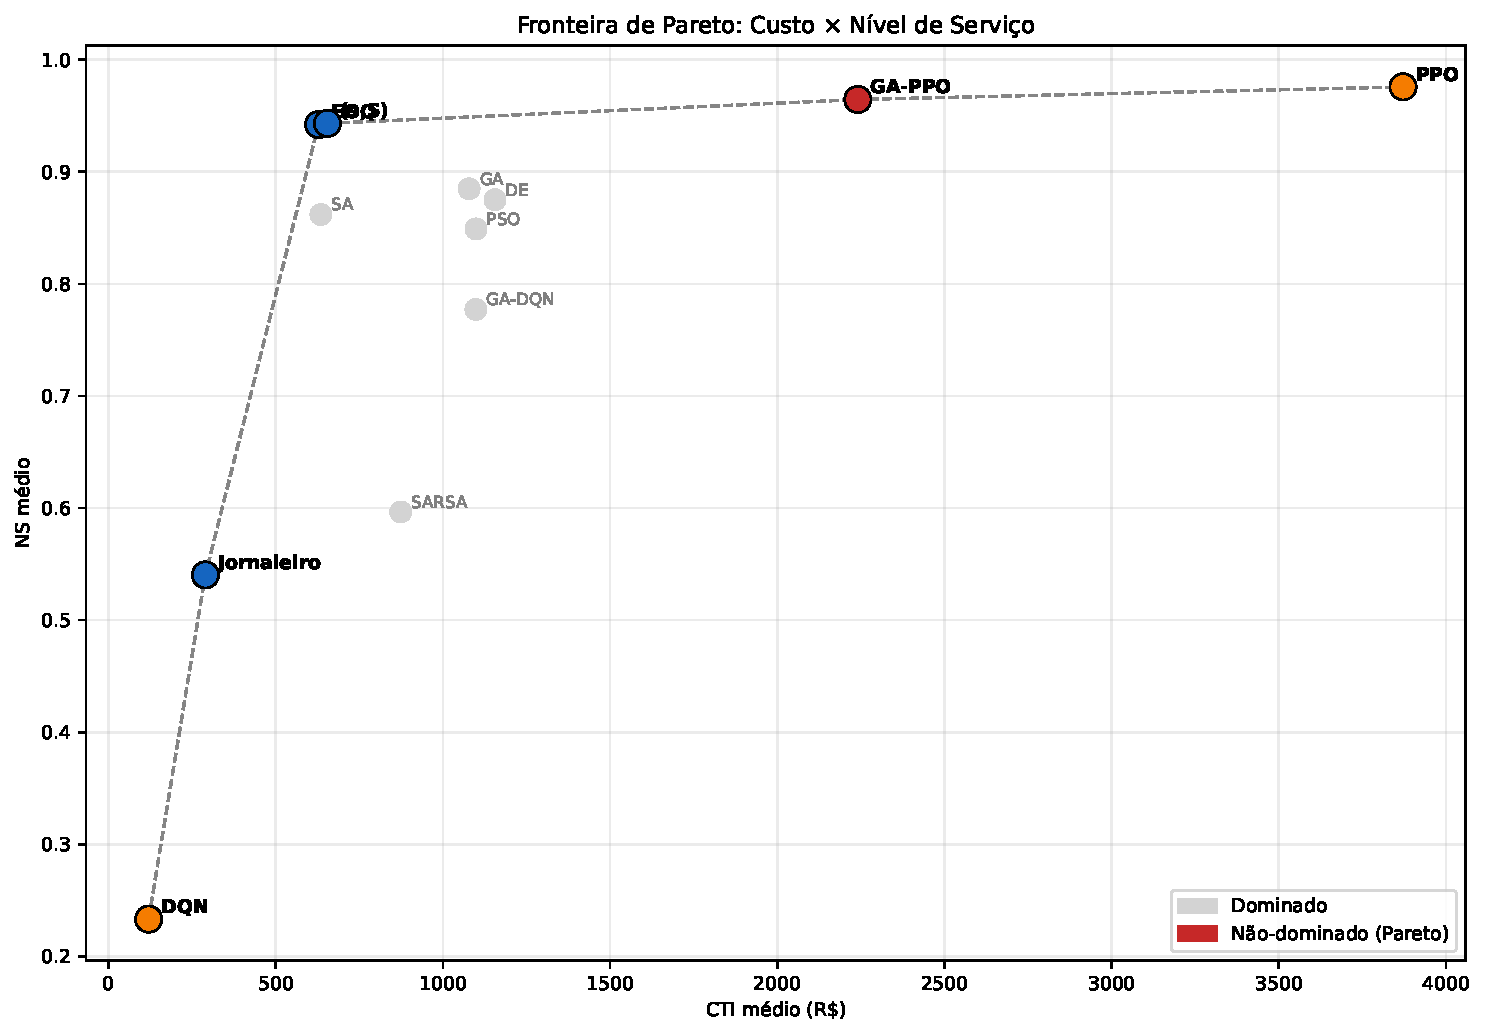
\includegraphics[width=\linewidth]{figures/pareto_frontier.pdf}\\
      \scriptsize Fronteira de Pareto CTI--NS
    \column{0.5\textwidth}
      \centering
      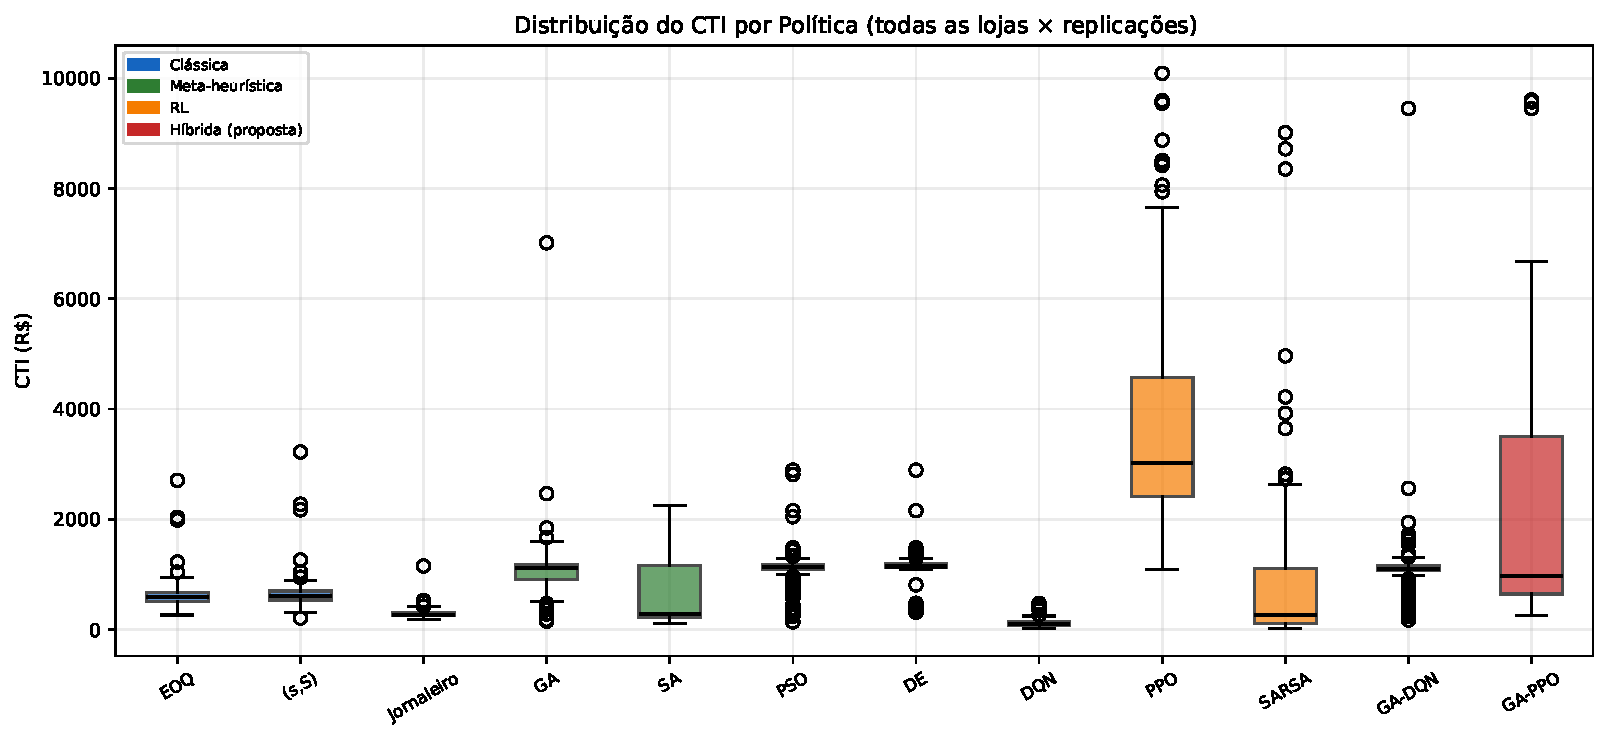
\includegraphics[width=\linewidth]{figures/boxplot_tic.pdf}\\
      \scriptsize Dispersão de CTI por política
  \end{columns}
  \vspace{0.5em}
  \small Sobre as 145 séries da Bahia: \highlight{EOQ} e $(s,S)$ oferecem o
  melhor equilíbrio custo-serviço agregado (NS\,$=$\,0,94); o
  \highlight{Jornaleiro} tem o menor custo bruto, mas NS\,$=$\,0,54.
  \note{
    Estas duas figuras resumem a evidência empírica central do Experimento
    2. À esquerda, a fronteira de Pareto entre CTI e NS mostra que nenhum
    ponto ocupa simultaneamente o menor custo e o maior nível de serviço --
    quem prioriza custo aponta para o Jornaleiro, quem prioriza serviço
    aponta para EOQ ou (s,S). À direita, o boxplot mostra que a mesma
    política produz custos muito diferentes entre séries -- a eficácia
    depende do perfil da demanda, não só da política escolhida. Essa
    heterogeneidade é a evidência empírica direta que justifica a
    necessidade de seleção contextual.
  }
\end{frame}
